\paragraph{}
Ker ne re"sujemo enostavnih problemov, potrebujemo zakomplicirati tudi samoumevne stvari kot so funkcije. Celo "zivljenje smo zapisovali funkcije kot $f(x)$. Ta zapis nam predstavlja funkcijo $f$, ki je odvisna od parametra $x$. To pomeni, da nam za vsak dani $x$ priredi novo "stevilko. "Ce "zelimo narisati graf take funkcije, uporabimo 2D koordinatni sistem in nanj nari"semo to"cke, ki nam jih vrne funkcija, to pomeni urejene pare $(x, f(x))$.

\paragraph{}
Ker pa smo v svobodni dr"zavi, nam ni prepovedano, da bi bila funkcija odvisna od ve"c parametrov. Funkcijo odvisno od dveh parametrov bi zapisali kot $f(x,y)$. Taki funkciji podamo 2 "stevilki, $x$ in $y$, vrne pa nam eno "stevilko. "Ce "zelimo narisati graf take funkcije potrebujemo 3D koordinatni sistem. Za vsak urejen par $(x,y)$, bi nam taka funkcija priredila novo "stevilko, ki bi v tem koordinatnem sistemu predstavljala vi"sino, to je vrednost na $z$ osi. Primer take funkcije je:
\[f(x,y) = \frac{\sin \sqrt{x^2 + y^2}}{\sqrt{x^2 + y^2}} \]

$\sqrt{x^2 + y^2}$ predstavlja oddaljenost to"cke, ki jo podamo funkciji, od izhodi"s"ca.

\begin{figure}[h!]
	\centering
	\caption{3D funkcija}
	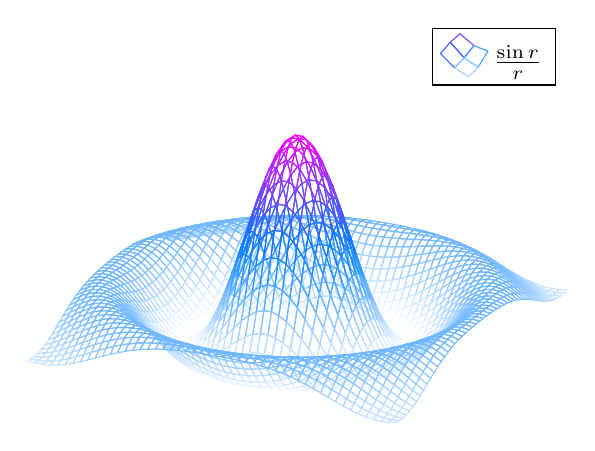
\begin{tikzpicture}
	\begin{axis}[
	hide axis,
	colormap/cool,
	]
	\addplot3[
		mesh,
		samples=50,
		domain=-8:8,
	]
	{sin(deg(sqrt(x^2+y^2)))/sqrt(x^2+y^2)};
	\legend{$\frac{\sin r}{r}$}
	\end{axis}
	\end{tikzpicture}
\end{figure}

\paragraph{}
Funkcija je seveda lahko odvisna tudi od ve"c kot dveh spremenljivk. Takih funkcij pa na na"so veliko "zalost ne moremo narisati, ker bi "ze za funkcijo odvisno od treh spremenljivk, potrebovali 4 dimenzionalni prostor.

\paragraph{}
Glede na to da smo "se vedno v svobodni dr"zavi, se lahko pri parametrih funkcije poigramo tudi z njihovim poimenovanjem. Nikjer ne pi"se, da ne smemo na mesto $x$ uporabljati $a$ in da na"sa funkcija ne sme izgledati kot $f(a)$. To seveda velja tudi za funkcije, ki vzamejo ve"cparametrov, tako da lahko namesto $f(x,y)$ pi"semo $f(a,b)$. Funkcijo katere graf je narisan od zgoraj, bi lahko potemtakem zapisali kot:
\[f(a,b) = \frac{\sin \sqrt{a^2 + b^2}}{\sqrt{a^2 + b^2}} \]

\paragraph{}
Definirali smo "ze napako premice za dane to"cke. Ker sedaj vemo, da je funkcija lahko odvisna od ve"cih spremenljivk in da ni nujno da sta ti spremenljivki $x$ in $y$, lahko ugotovimo, da je na"sa napaka funkcija, ki je odvisna od spremenljivk $a$ in $b$. Druga"ce seveda ne more biti, ker imamo skupino to"ck "ze podano, to pomeni $(x_1, y_1), (x_2, y_2) \ldots$, za katere "zelimo najti premico, ki se jim prilega, tako da lahko v na"si funkciji napake spreminjamo samo parametra $a$ in $b$.
